% Chapter 1

\chapter{Adversarial Networks Training} % Main chapter title
\label{Chapter5} % For referencing the chapter elsewhere, use \ref{Chapter1} 

Now that we built our dataset, we have the data we need to proceed with the generative part of our pipeline.

It is once again important to place this chapter in the context of our data pipeline, as we introduced it in section~\ref{sec:datapipeline} and as we show it in figure~\ref{fig:pipeline}. The dataset we just created is composed of policies (which are just tables or 2D matrices).  More specifically we have 3,827 such policies, corresponding to all the 3,827 different valid map configurations of our environment, \code{RandomisedFrozenLake}. We split the dataset in a training subset (80\%) of the total number of policies, and the test subset (the remaining 20\%).

In section~\ref{sec:gan} we introduced Generative Adversarial Networks, detailing their vanilla architecture, as they were introduced by \citeauthor{goodfellow2014generative}. We now build off of this architecture to build a GAN architecture for policy generation.

In this section we present such architecture, explain the design decisions that were involved in configuring it, and describe the process of training it in an adversarial manner. We also provide a detailed breakdown of the generator and the discriminator's deep neural networks.

The input to our Policy GAN will only be the training subset of the policies we trained with Q-learning. In this way, we hope to be able to model, through our GAN, a distribution on these policies such that we can capture knowledge that we can transfer to other unseen tasks.
These unseen tasks are exactly the ones corresponding to the map configurations of the test substed, and we therefore do not include those policies as our input to our GAN.

%----------------------------------------------------------------------------------------

\section{Policy GAN}
In figure~\ref{fig:PolicyGAN} we show the architecture of our Policy GAN.
We already described most of the details involved when training GANs in section~\ref{sec:gan}. 

Training a GAN is an iterative process that runs for a set amount of epochs (an epoch is one full training cycle on the training set).
At each iteration, the mini-batch inputs to the discriminator \code{D} are taken from both the real data sampled from the training data (in our case policies from the training set that we created in chapter~\ref{Chapter4}), and the samples generated by the generator.
Given \code{D}'s prediction, we then apply a gradient-based optimisation method to update both \code{D}'s and \code{G}'s parameters.

Building neural net architecture that work well in practice generally involves finding and tuning many parameters and making several design decisions that make the issue not trivial.


\begin{figure}
\centering
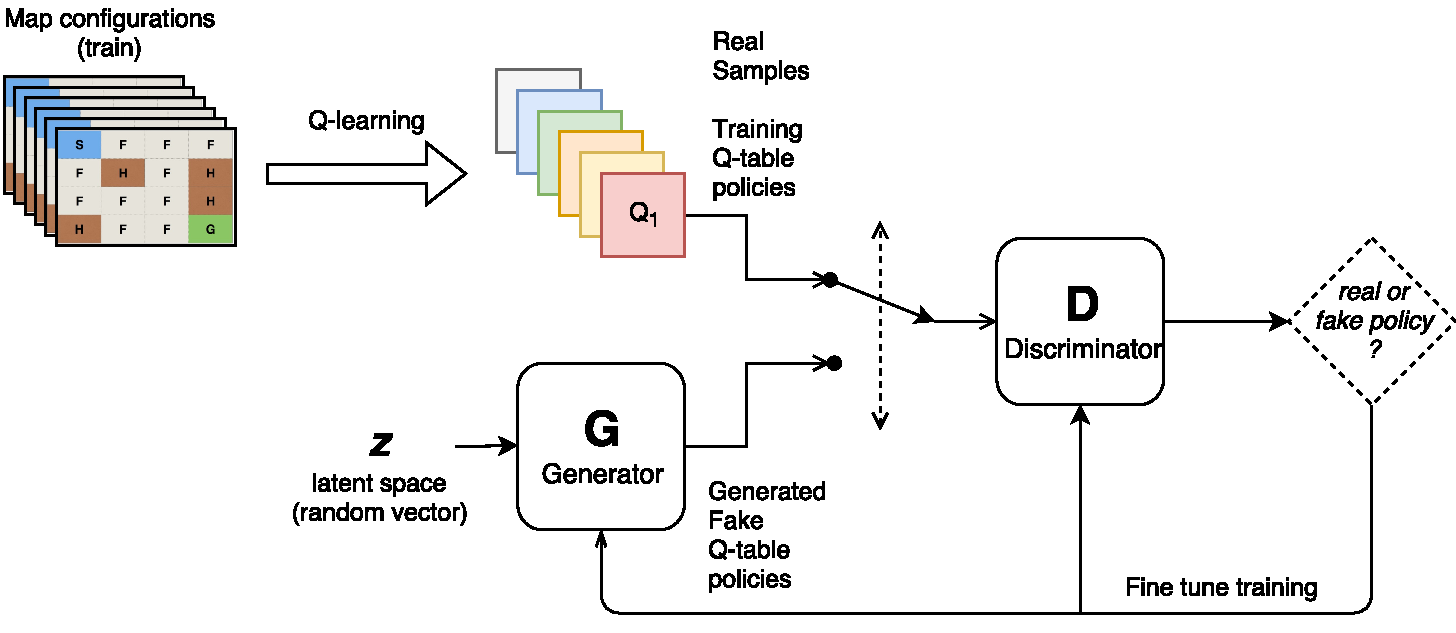
\includegraphics[width=15cm]{Figures/PolicyGAN}
\caption{Our Policy GAN architecture}
\label{fig:PolicyGAN}
\end{figure}

\subsection{Gradient descent optimisation}
Learning rates have historically been one of the trickiest hyperparameters to set, as it drastically influences the final results, perhaps more than all other hyperparameters.

Gradient descent \citep{lemarechal2012cauchy}, a seminal approach to optimisation that dates back to Cauchy a few centuries back, still proves relatively successful in many machine learning applications.
Since then, a lot of work has been put in devising algorithms that have adaptive learning rates and that lead to faster convergence, and we here report examples of two such algorithms: RMSProp \citep{hinton2012neural} and Adam \citep{DBLP:journals/corr/KingmaB14}

In this section we introduce and compare RMSProp and Adam with gradient descent as the different learning rules we could use in our classification task. Both perform local optimisation with different techniques and metrics that are constructed from the history of previous iteractions.

The former (algorithm \ref{alg:RMSProp}) is a modification of the AdaGrad optimiser \citep{duchi2011adaptive}, that modifies the gradient accumulation into a moving average that is exponentially weighted.

The latter (algorithm \ref{alg:Adam}) is best described as a combination of RMSProp and SGD with momentum \citep{sutskever2013importance}. Momentum accelerates SGD by multiplying the learning rate by a parameter that increases as we go towards the right direction in the gradient update.


%----------------------------------------------------------------------------------------


\section{Generator}
Figure~\ref{fig:Generator} shows the 

\subsection{Activation functions}

\subsection{Batch Normalisation}
Batch Normalisation \citep{DBLP:journals/corr/IoffeS15} is a technique that improves stability and performance of neural networks by normalising the inputs of each layer such that they have a mean output activation of zero and standard deviation of one. Benefits of using batch normalisation include faster training time (i.e. faster convergence to optimal model). This also allows higher learning rates and weight initialisation won't be as critical.

We first compute the mean and variance of each hidden unit activation across the minibatch (size $M$):
\begin{gather*}
\mu_i \leftarrow \frac{1}{M} \sum_{m=1}^{M}u_i^m \\
\sigma_i^2 \leftarrow \frac{1}{M} \sum_{m=1}^{M}(u_i^m - \mu_i)^2
\end{gather*}

The result of doing batch normalisation will then be:
\begin{gather*}
u_i = w_ix \\
\hat{u_i} = \frac{u_i-\mu_i}{\sqrt{\sigma_i^2 + \epsilon}} \\
z_i = \gamma_i\hat{u_i}+\beta_i = \text{batchNorm}({u_i})
\end{gather*}

where $\gamma$ and $\beta$ are parameters updated with gradient descent that will scale and shift the normalised activations.


\begin{figure}
\centering
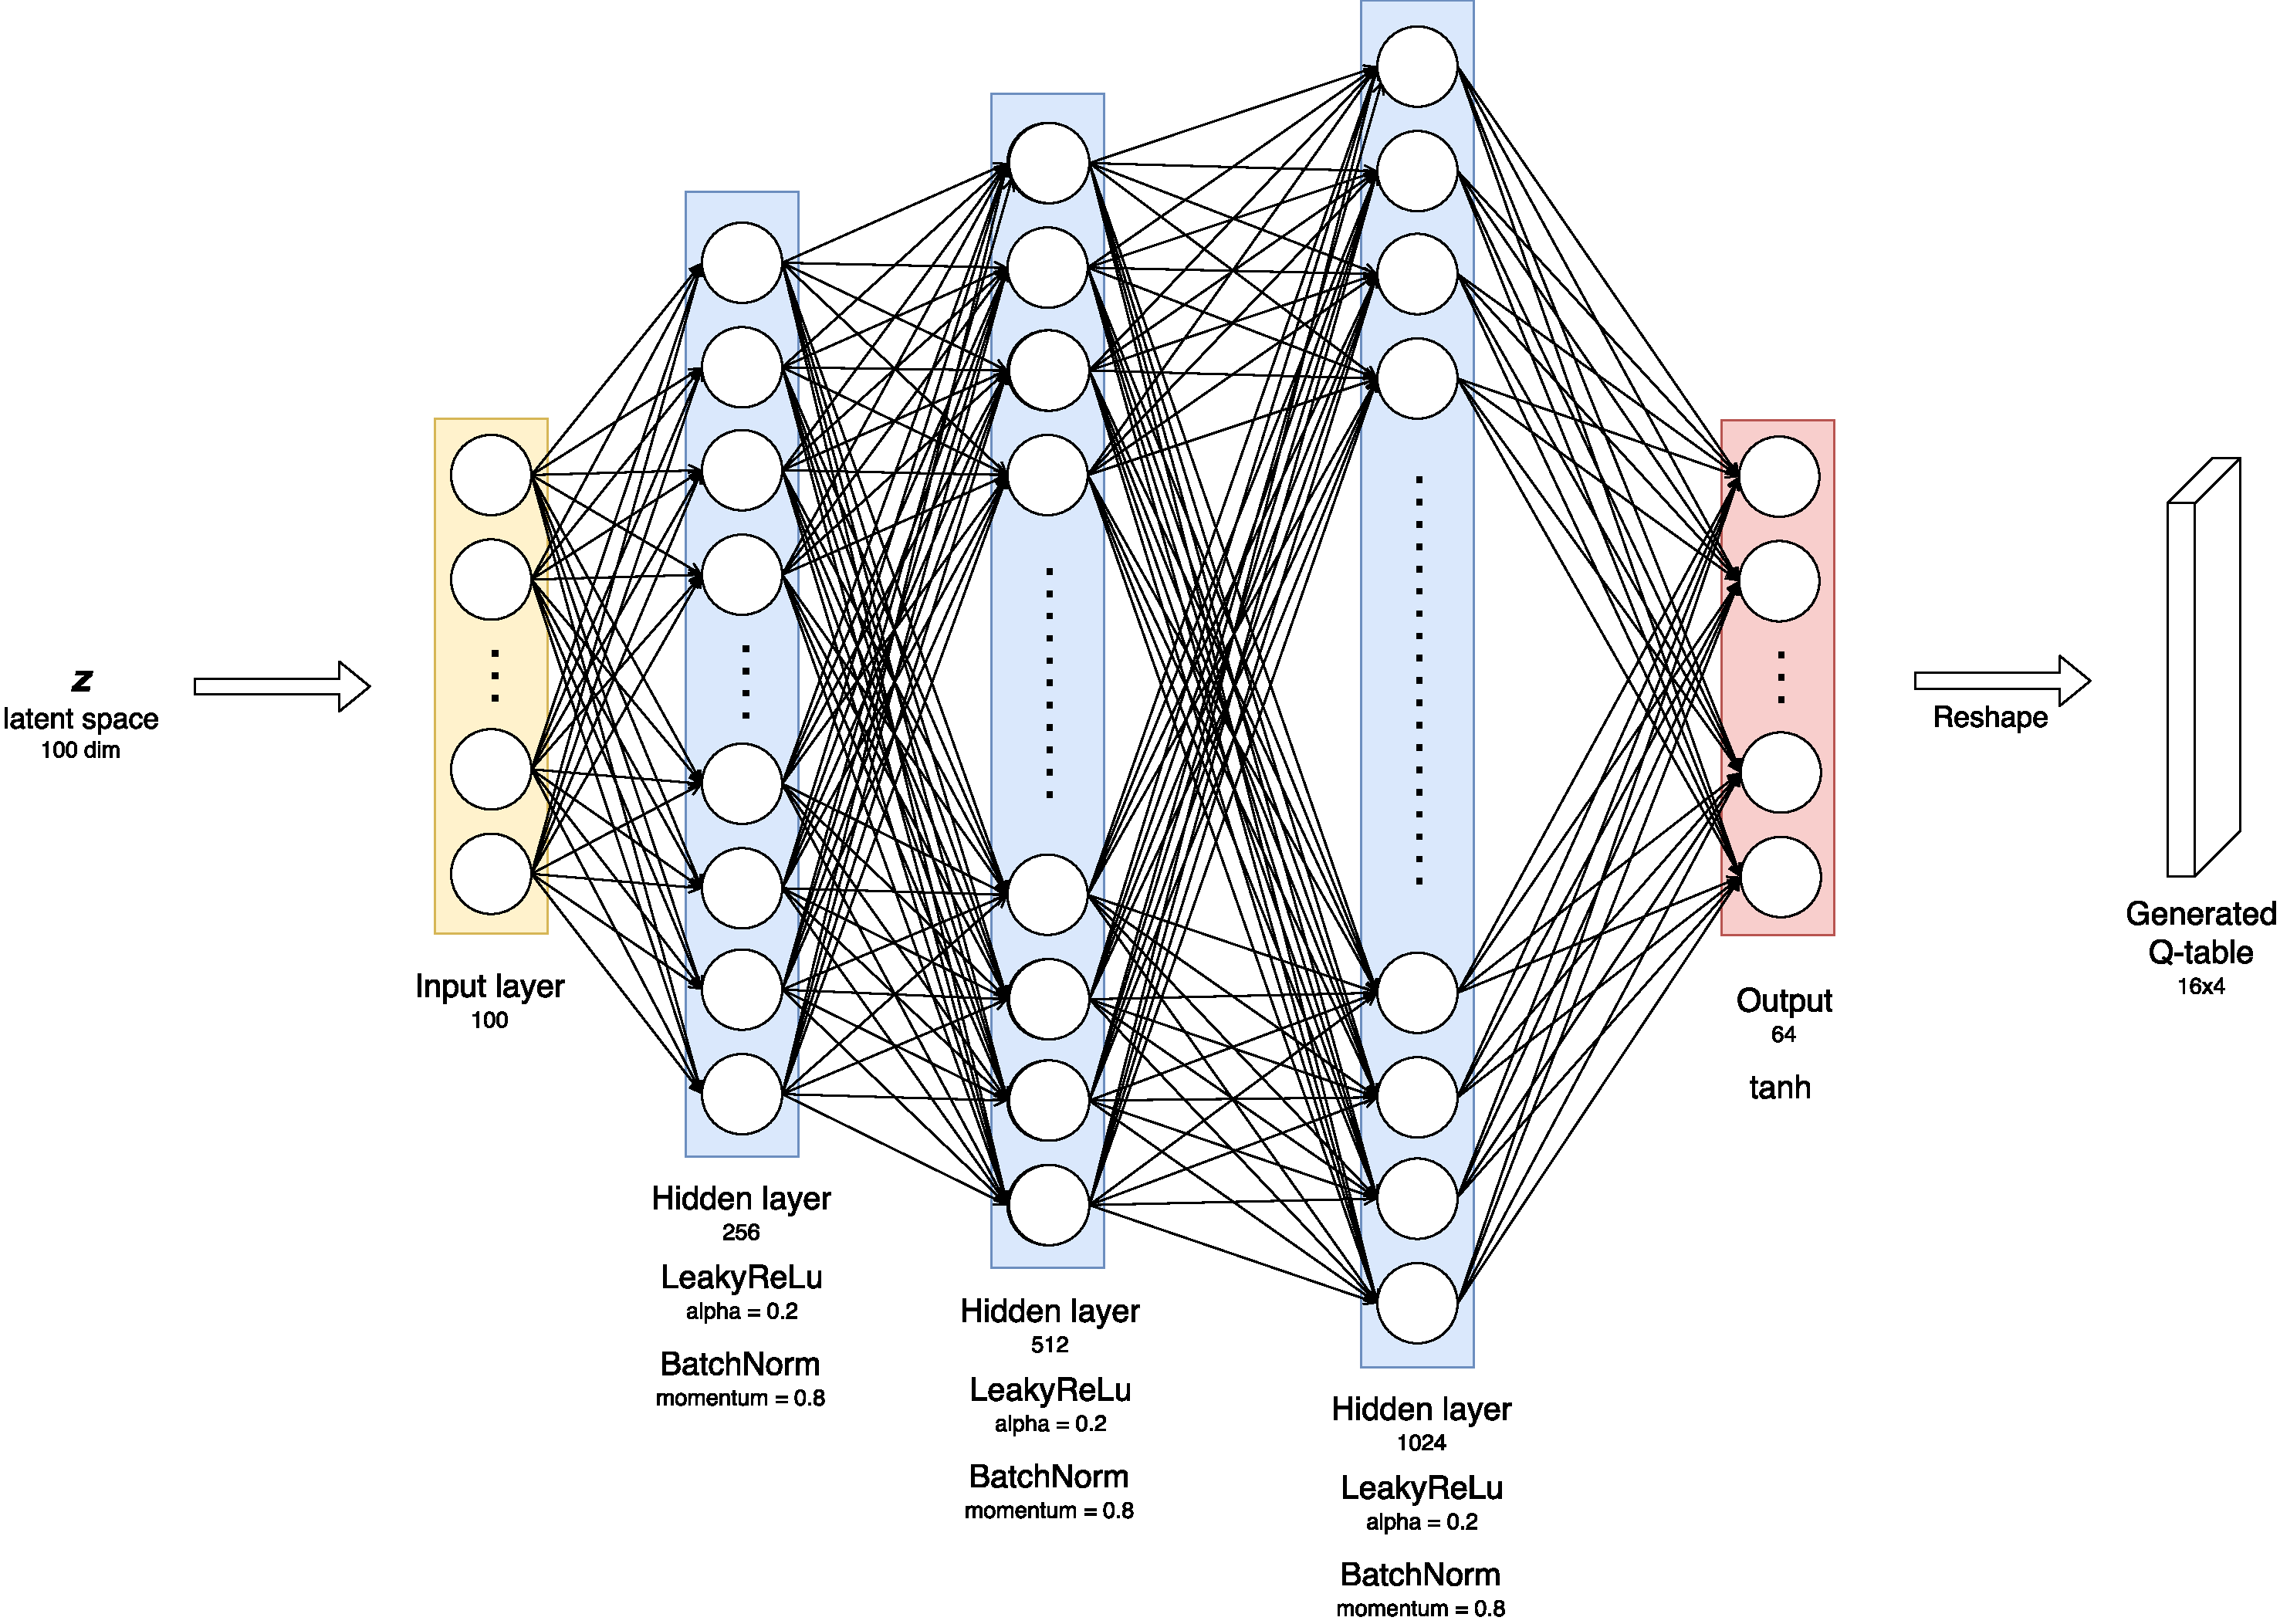
\includegraphics[width=15cm]{Figures/Generator}
\caption{Architecture of the Generator network}
\label{fig:Generator}
\end{figure}

%----------------------------------------------------------------------------------------

\section{Discriminator}
\begin{figure}
\centering
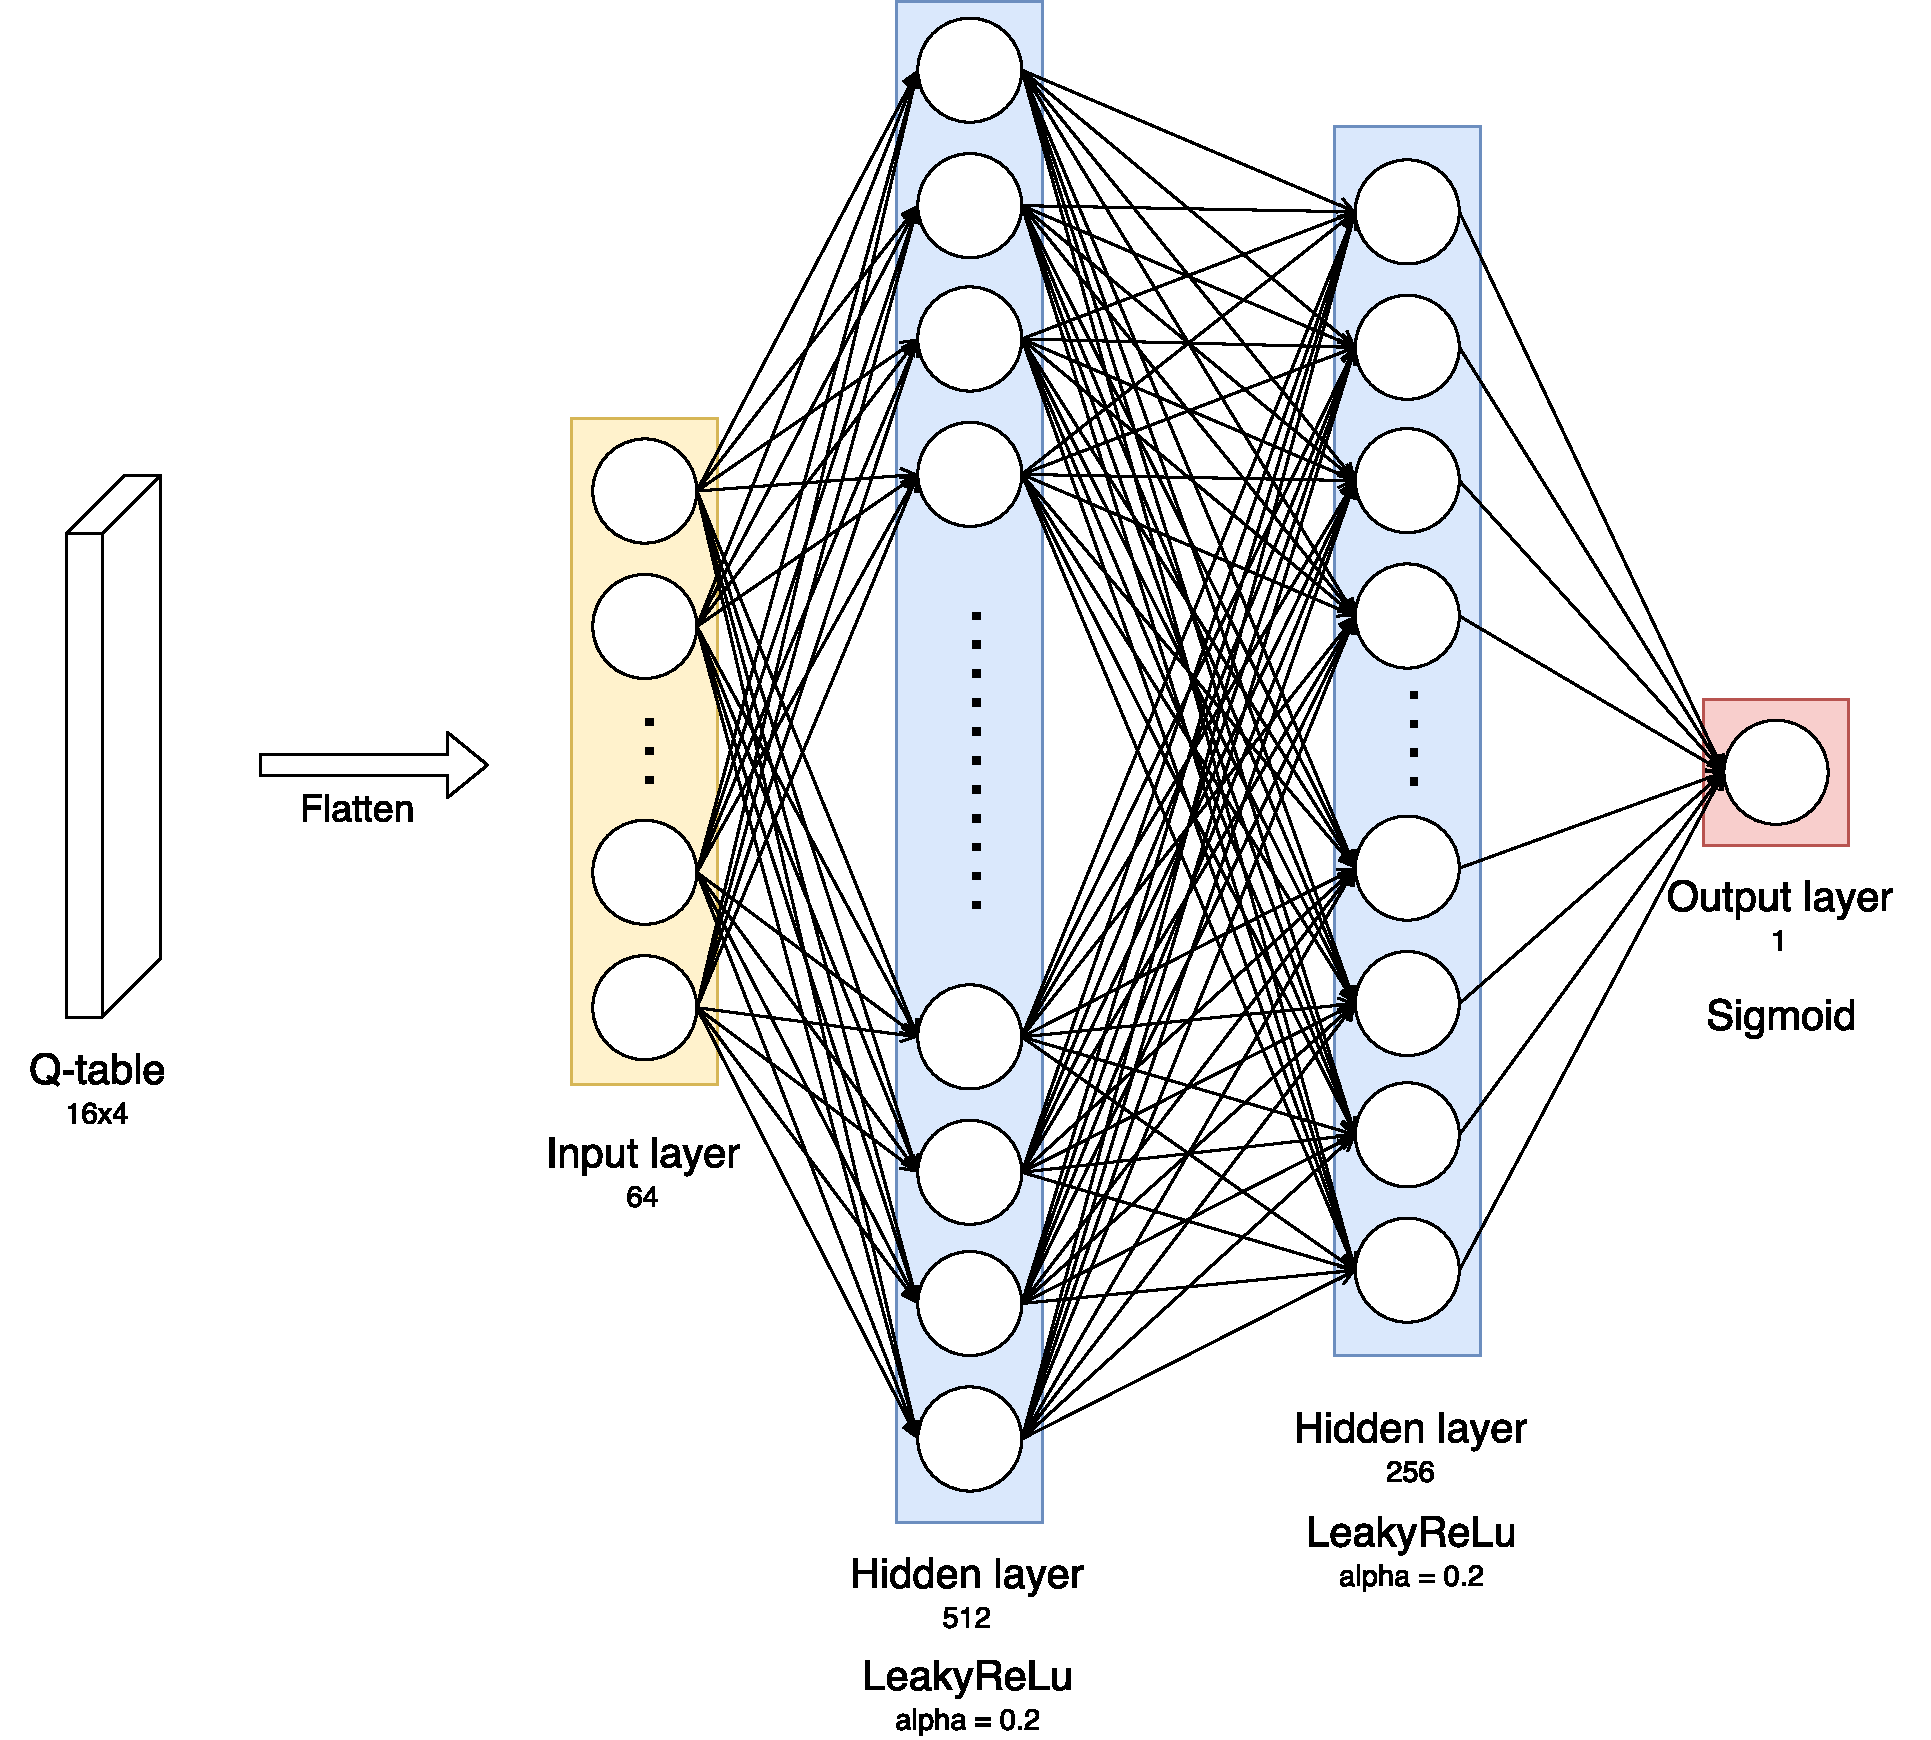
\includegraphics[width=10cm]{Figures/Discriminator}
\caption{Architecture of the Discriminator network}
\label{fig:Discriminator}
\end{figure}